%%%%%%%%%%%%%%%%%%%%%%%%%%%%%%%%%%%%%%%%%%%%%%%%%%%%%%%%%%%%%%%%%%
%%%                      Homework _                            %%%
%%%%%%%%%%%%%%%%%%%%%%%%%%%%%%%%%%%%%%%%%%%%%%%%%%%%%%%%%%%%%%%%%%

\documentclass[letter]{article}

\usepackage{lipsum}
\usepackage[pdftex]{graphicx}
\usepackage[margin=1.5in]{geometry}
\usepackage[english]{babel}
\usepackage{listings}
\usepackage{amsthm}
\usepackage{amssymb}
\usepackage{framed} 
\usepackage{amsmath}
\usepackage{titling}
\usepackage{fancyhdr}

\pagestyle{fancy}


\newtheorem{theorem}{Theorem}
\newtheorem{definition}{Definition}

\newenvironment{menumerate}{%
  \edef\backupindent{\the\parindent}%
  \enumerate%
  \setlength{\parindent}{\backupindent}%
}{\endenumerate}







%%%%%%%%%%%%%%%
%% DOC INFO %%%
%%%%%%%%%%%%%%%
\newcommand{\bHWN}{1}
\newcommand{\bCLASS}{CS189}

\title{\bCLASS: Homework \bHWN}
\author{William Guss\\26793499\\wguss@berkeley.edu}

\fancyhead[L]{\bCLASS}
\fancyhead[CO]{Homework \bHWN}
\fancyhead[CE]{GUSS}
\fancyhead[R]{\thepage}
\fancyfoot[LR]{}
\fancyfoot[C]{}
\usepackage{csquotes}

%%%%%%%%%%%%%%

\begin{document}
\maketitle
\thispagestyle{empty}


%%%%%%% Be sure to set the counter and use menumerate
Here is the first graph. It has the error rate. \\
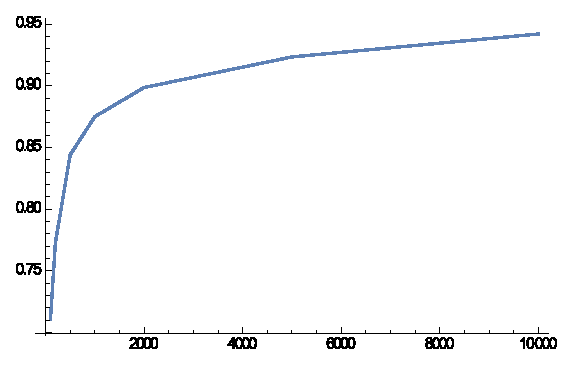
\includegraphics{GRAPHS_gr1.eps}

Here are the confusion matrices.\\
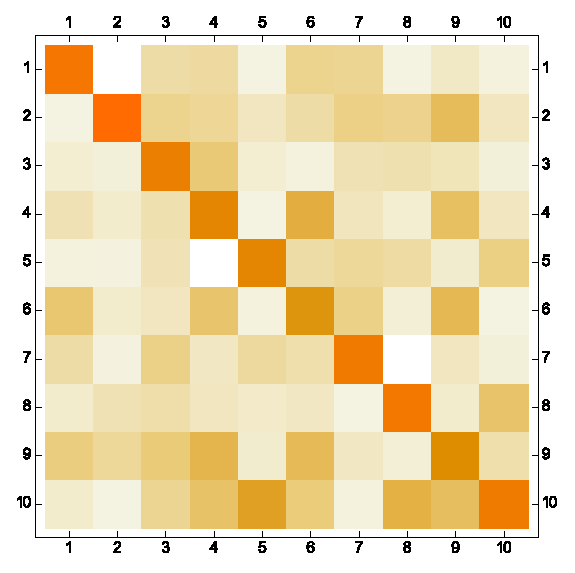
\includegraphics{GRAPHS_gr2.eps}

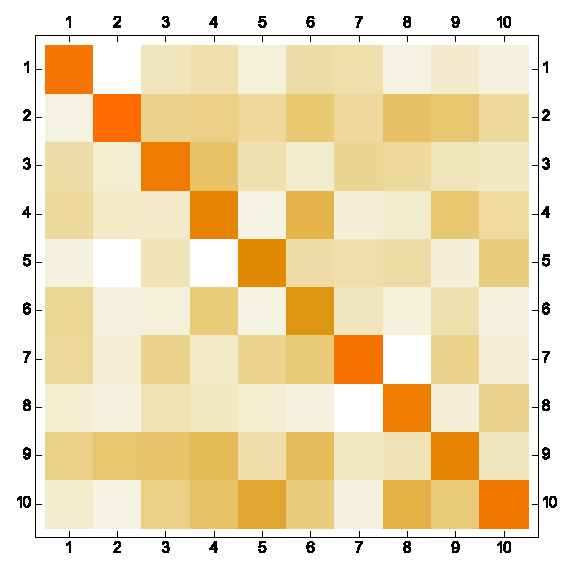
\includegraphics{GRAPHS_gr3.eps}

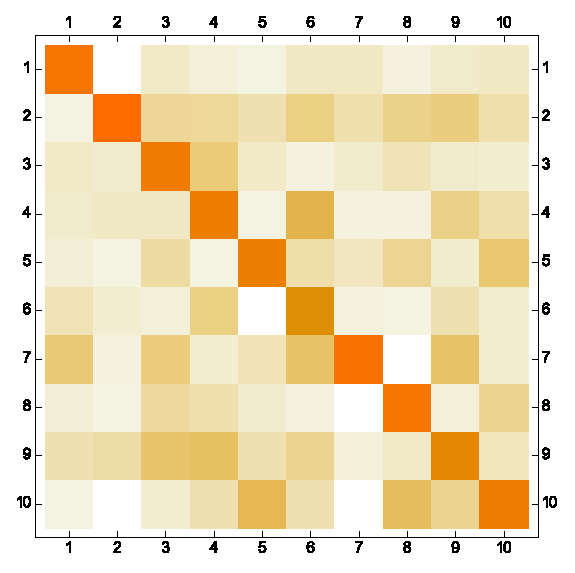
\includegraphics{GRAPHS_gr4.eps}

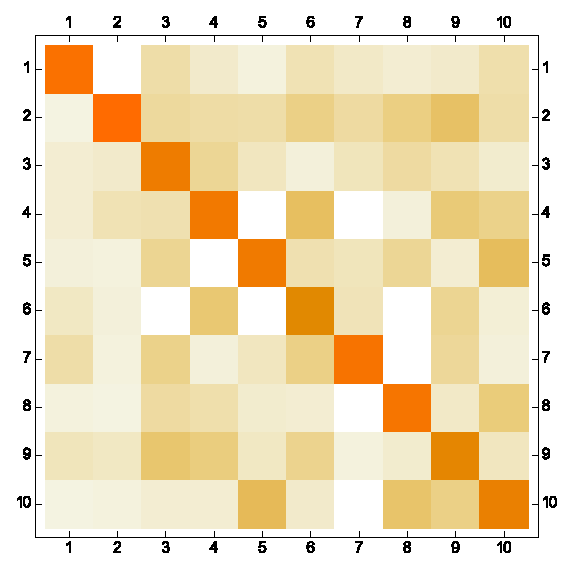
\includegraphics{GRAPHS_gr5.eps}

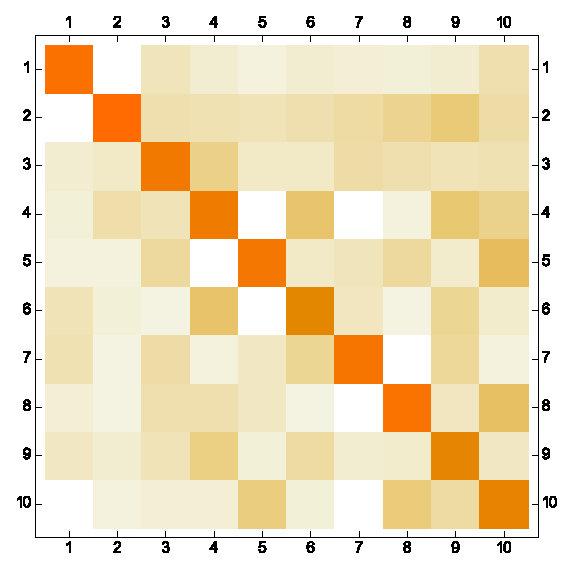
\includegraphics{GRAPHS_gr6.eps}

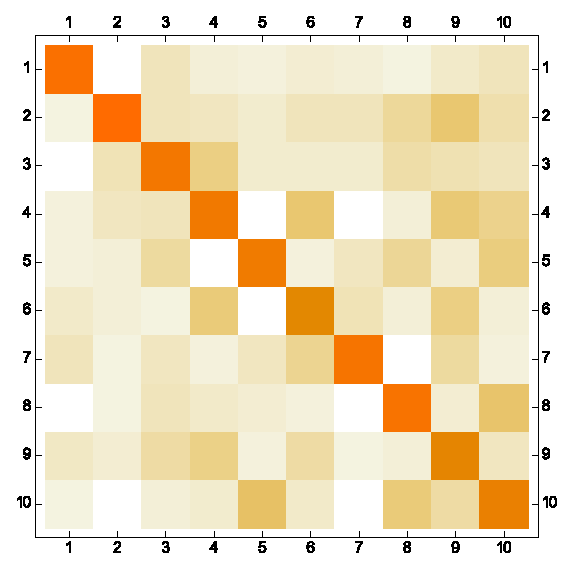
\includegraphics{GRAPHS_gr7.eps}

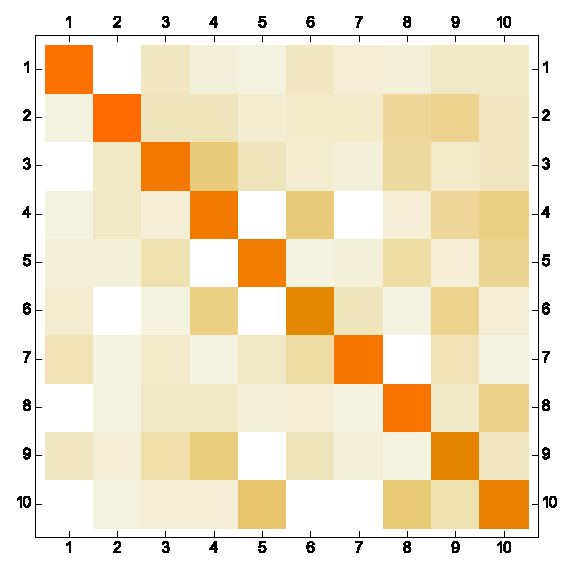
\includegraphics{GRAPHS_gr8.eps}

The confusion matrices tend towards one whose diagonals are
largely the largest values as training happens. This makes sense since it misclassifies less.

The value I got for $C$ with iterated application of a binary search on $10-fold$ classification with $10000$ values was $2.93.$
\end{document}